\subsection{实际应用性能}
\label{socksdirect:subsec:application}


本节演示了\sys {}可以在不修改代码的情况下显着提高实际应用程序的性能。
Rsocket~ \cite {rsockets}与以下任何应用程序都不兼容。

\subsubsection{Nginx HTTP 服务器}



为了测试客户端来自网络并在主机内提供服务的典型Web服务方案,本节使用Nginx~ \cite {nginx} v1.10作为HTTP请求生成器和HTTP响应生成器之间的反向代理。
Nginx和响应生成器位于同一主机中,而请求生成器位于不同的主机中。
生成器使用保持活动的TCP连接与Nginx进行通信。
由于fork,LibVMA~ \cite {libvma}不能与未修改的Nginx一起使用。
在图 \ref {socksdirect:fig:eval-nginx}中,请求生成器测量从发送HTTP请求到接收整个响应的时间。
对于较小的HTTP响应大小,与Linux相比,\sys {}可将延迟减少5.5倍。
对于大型响应,由于零拷贝,\sys {}可将延迟降低多达20倍。

\begin{figure}[htbp]
	\centering 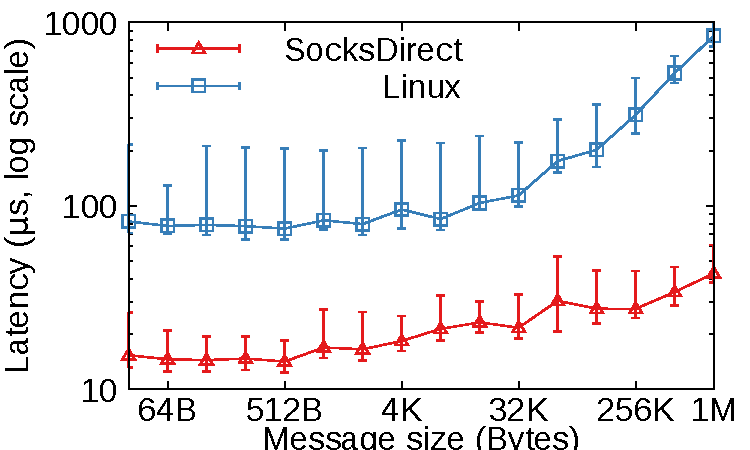
\includegraphics[width=0.5\textwidth]{eval/web/msgsize-clocal-lat.pdf}
	
	\caption{Nginx HTTP 请求端到端延迟。}
	\label{socksdirect:fig:eval-nginx}
\end{figure}


%In Figure B, to test the how Nginx throughput scales with multiple cores, we run Nginx with a fixed number of worker threads and response size 1KB.
%The request generator sends multiple HTTP requests in parallel, and we use a sufficient number of generator threads to saturate Nginx throughput.
%Figure B: throughput scalability with number of cores.

\subsubsection{Redis 键值存储}

本节使用redis-benchmark客户端和8字节GET请求来测量Redis~ \cite {redis} 内存键值存储服务器的延迟。
使用Linux时,平均延迟为38.9 $ \mu s $,1%和99%百分位延迟分别为31.6和56.1 $ \mu s $。
使用\sys {} 后,平均延迟为14.1 $ \mu s $(比Linux低64%),1 %和99 %百分位数8.4和19.1 $ \mu s$。

%Figure: line chart, y axis: throughput, lines: (intra-, inter-) x (\sys{}, libvma, Linux). x axis: number of concurrent clients.

%Utility: redis-benchmark.
%Key point: concurrency low: test latency, concurrency high: test throughput.

%\subsection{Real-time Stream Processing}

%Apache Flink~\cite{carbone2015apache} (need to turn off durability on disk)

%Scenario: Word Count (distributed system with one source, two mappers and one reducer)

%Metrics: Latency, throughput

\subsubsection{远程过程调用(RPC)库}

本节使用RPClib~ \cite {rpclib}来测量RPC延迟。
在主机内的两个进程中运行RPClib中的示例1~KiB RPC,需要45 $ \mu $s。 在两个主机上,RPC需要79 $ \mu$s。
使用\sys {},主机内延迟变为21 $ \mu s $(减少53%),主机间为46 $ \mu$s (减少42%)。

然而,\sys{} 不是万能药。即使使用了 \libipc{}, RPClib 的性能仍然远远低于最先进的 RPC 库,如 eRPC \cite{kalia2018datacenter},由于 RPClib 的开销成为性能瓶颈。

\subsubsection{网络功能流水线}

\emph {pcap}格式的64字节数据包来自外部数据包生成器,通过网络功能(NF)管道,并发送回数据包生成器。
本节将每个NF实现为一个进程,它从\emph {stdin}输入数据包,更新本地计数器,并输出到\emph {stdout}。
对于Linux,使用\emph {pipe}和\emph {TCP socket}来连接主机内的NF进程。
图 \ref {socksdirect:fig:eval-tun-tput}表明\sys {}的吞吐量分别是Linux管道和TCP套接字的15倍和20倍。
它甚至接近最先进的NF框架,NetBricks~ \cite {panda2016netbricks}。

\begin{figure}[htbp]
	\centering
	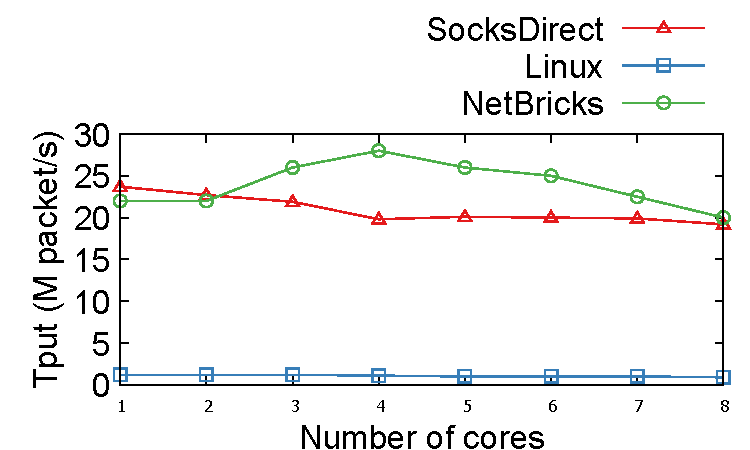
\includegraphics[width=0.5\textwidth]{eval/microbenchmark/nfv-tun-tput.pdf}
	
	\caption{网络功能流水线的吞吐量。}
	\label{socksdirect:fig:eval-tun-tput}
	%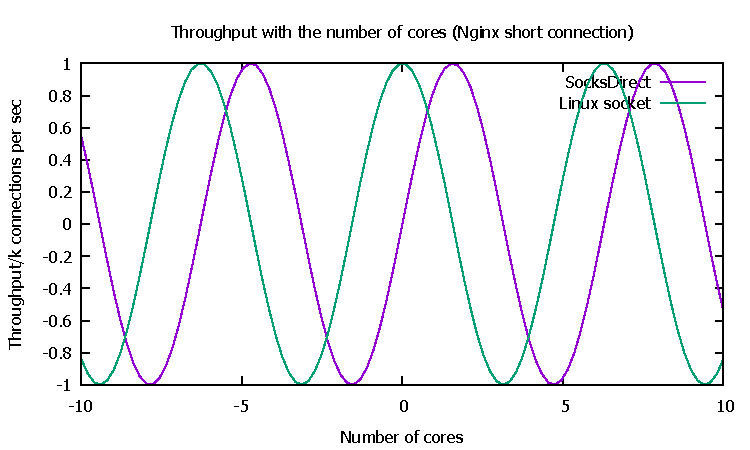
\includegraphics[width=\textwidth]{eval/microbenchmark/nginx-short-tput.pdf}
	%
	%\label{socksdirect:fig:eval-nginx-short}
	%\caption{Nginx throughput.}
	
	%\centering 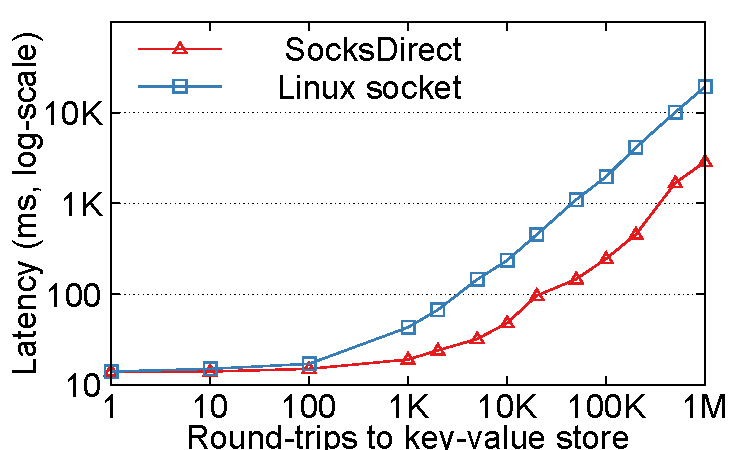
\includegraphics[width=\textwidth]{eval/microbenchmark/nginx-multiround-tput.pdf}
	%
	%\caption{End-to-end HTTP request latency of a web service.}
	%\label{socksdirect:fig:eval-nginx-multiround}
	
	%\centering
	%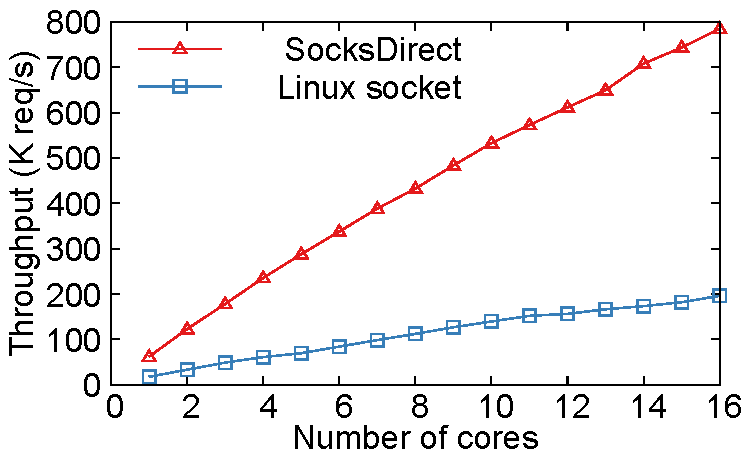
\includegraphics[width=\textwidth]{eval/microbenchmark/corenum-http-tput.pdf}
	%
	%\caption{Multi-core scalability of HTTP backend service throughput.}
	%\label{socksdirect:fig:eval-http-tput}
\end{figure}


%\subsubsection{GraphX on Spark}
%\quad

%Two nodes run distributed PageRank.
%Test elapsed time per iteration with \sys{}, libvma and Linux. (Only need three numbers, no figure.)
